\documentclass[runningheads]{llncs}
\usepackage{xcolor}
\usepackage{amsmath}
\usepackage{tikz}
\usetikzlibrary{arrows.meta, chains, fit, positioning}

\newcommand{\smallfont}{\fontsize{1pt}{1.2pt}\selectfont}

\begin{document}

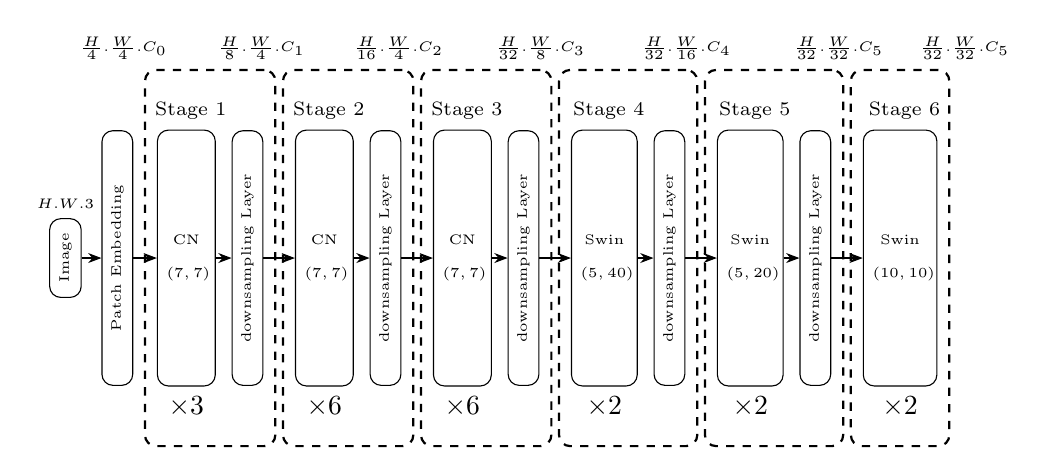
\begin{tikzpicture}[
start chain = going right,
windowedsmall/.style = {rounded corners, draw, %fill=gray!20,
                  text width=0.6cm,align=flush center, %left,
                  on chain, join=by line,
                  minimum height=3.25cm,
                  minimum width=0.7cm,
                  inner ysep=7.5ex},
windowedbig/.style = {rounded corners, draw, %fill=gray!20,
                  text width=0.7cm,
                  align=flush center, %left,
                  on chain, join=by line,
                  minimum height=3.25cm,
                  minimum width=0.7cm,
                  inner ysep=7.5ex},
convnext/.style = {rounded corners, draw, %fill=gray!20,
                  text width=0.5cm,align=flush center, %left,
                  on chain, join=by line,
                  minimum height=3.25cm,
                  minimum width=0.6cm,
                  inner ysep=7.5ex},
vertical/.style = {rounded corners, draw, %fill=gray!20,
                  text width=3cm, align=flush center, %left,
                  minimum height=.05cm,
                  minimum width=3cm,
                  on chain, join=by line},
stage/.style={draw, rounded corners, thick, dashed, inner ysep=4ex, inner xsep=2ex, yshift=1ex},
line/.style = {-Stealth}
                    ]
%%% NODES %%%
\node (n1) [draw, rotate=90,anchor=north, rounded corners, on chain, join=by line, minimum height=.4cm, minimum width=1cm, label=0:{ \smallfont  $H$.$W$.$3$}] {\smallfont Image};
\node (n2) [vertical, rotate=90, right=.25cm of n1.south, anchor=north] {\smallfont Patch Embedding};

\node (n3) [convnext, right=.3cm of n2.south, label=270:{$\times3$}, label=88:{\scriptsize Stage 1}] {\smallfont CN \\  $(7,7)$};
\node (n4) [vertical, rotate=90, right=.2cm of n3, anchor=north] {\smallfont downsampling Layer}; 

\node (n5) [convnext, right=.4cm of n4.south, label=270:{$\times6$}, label=88:{\scriptsize Stage 2}] {\smallfont CN\\  $(7,7)$};
\node (n6) [vertical, rotate=90, right=.2cm of n5, anchor=north] {\smallfont downsampling Layer};

\node (n7) [convnext, right=.4cm of n6.south, label=270:{$\times6$}, label=88:{\scriptsize Stage 3}] {\smallfont CN \\  $(7,7)$};
\node (n8) [vertical, rotate=90, right=.2cm of n7, anchor=north] {\smallfont downsampling Layer};

\node (n9) [windowedsmall,  right=.4cm of n8.south, label=270:{$\times2$}, label=88:{\scriptsize Stage 4}] {\smallfont Swin \\   $(5,40)$};
\node (n10) [vertical, rotate=90, right=.2cm of n9, anchor=north] {\smallfont downsampling Layer};

\node (n11) [windowedsmall, right=.4cm of n10.south, label=270:{$\times2$}, label=88:{\scriptsize Stage 5}] {\smallfont Swin \\  $(5,20)$};
\node (n12) [vertical, rotate=90, right=.2cm of n11, anchor=north] {\smallfont downsampling Layer};

\node (n13) [windowedbig, right=.4cm of n12.south, label=270:{$\times2$},label=88:{\scriptsize Stage 6}] {\smallfont Swin \\$(10,10)$};

 
 
%%% dotted RECTANGLE %%%
\node [draw, rounded corners, thick, dashed, align=center, inner ysep=5ex, inner xsep=1ex, yshift=0ex, fit=(n3) (n4), label=100:{\smallfont $\frac{H}{4}.\frac{W}{4}.C_0$}] (box) {};

\node[draw, rounded corners, thick, dashed, inner ysep=5ex, inner xsep=1ex, fit=(n5) (n6), label=100:{\smallfont $\frac{H}{8}.\frac{W}{4}.C_1$}] (box) {};

\node[draw, rounded corners, thick, dashed, inner ysep=5ex, inner xsep=1ex, fit=(n7) (n8), label=100:{\smallfont $\frac{H}{16}.\frac{W}{4}.C_2$}] (box) {};

\node[draw, rounded corners, thick, dashed, inner ysep=5ex, inner xsep=1ex, fit=(n9) (n10), label=100:{\smallfont $\frac{H}{32}.\frac{W}{8}.C_3$}] (box) {};

\node[draw, rounded corners, thick, dashed, inner ysep=5ex, inner xsep=1ex, fit=(n11) (n12), label=100:{\smallfont $\frac{H}{32}.\frac{W}{16}.C_4$}, label=87:{\smallfont $\frac{H}{32}.\frac{W}{32}.C_5$}] (box) {};
\node[draw, rounded corners, thick, dashed, inner ysep=5ex, inner xsep=1ex, fit=(n13), label=87:{\smallfont $\frac{H}{32} .\frac{W}{32}.C_5$}] (box) {};


\end{tikzpicture}

\end{document}